% Slide trình bày Bài #1 (tiếng Việt), khung "thiết kế ngược trước, nguyên tắc
% là cơ chế" (2026-10-08). Mọi số liệu lấy từ ../main_vi.tex (pipeline không
% cân bằng cạnh tuần hoàn, trừ kiểm định đặt trước P1.8 giữ bản gốc).
% Build: tectonic slides_vi.tex   (XeTeX, font nạp theo tên file .otf)
\documentclass[aspectratio=169,11pt]{beamer}

\usepackage{fontspec}
\setsansfont{texgyreheros}[Extension=.otf,UprightFont=*-regular,BoldFont=*-bold,ItalicFont=*-italic,BoldItalicFont=*-bolditalic]
\usepackage[vietnamese]{babel}
\usepackage{amsmath,amssymb}
\usepackage{graphicx}
\usepackage{booktabs}
\usepackage{tikz}
\usetikzlibrary{arrows.meta,positioning,fit}
\graphicspath{{../figures/}}
% Style TikZ đặt ở preamble: tham số #1 bên trong frame beamer gây lỗi \iterate.
\tikzset{
  box/.style={draw, rounded corners=2pt, align=center, font=\footnotesize,
              minimum height=11mm, inner sep=3pt, fill=#1},
  box/.default=white,
  arr/.style={-{Stealth[length=2mm]}, thick}}

\usetheme{Madrid}
\usecolortheme{default}
\usefonttheme{professionalfonts}
\setbeamertemplate{navigation symbols}{}
\setbeamertemplate{caption}{\raggedright\insertcaption\par}

\newcommand{\nuot}{\nu_{12}}
\newcommand{\nuto}{\nu_{21}}
\newcommand{\RR}{R^2}
% Màu nhấn dùng chung: đạt / không đạt
\newcommand{\pass}{\textcolor{green!50!black}{\textbf{đạt}}}
\newcommand{\fail}{\textcolor{red!70!black}{\textbf{không đạt}}}

\title[Tối ưu chính cái được kiểm chứng]{Tối ưu chính cái được kiểm chứng}
\subtitle{Tinh chỉnh không gian ẩn nhận biết nhị phân hóa cho thiết kế
ngược vật liệu meta auxetic bằng mô hình sinh}
\author[Trịnh Bình Minh]{Trịnh Bình Minh\\[2pt]
  {\small Hướng dẫn: GS.TS. Nguyễn Đình Đức}}
\date{08/10/2026}

\AtBeginSection[]{\begin{frame}{Nội dung}\tableofcontents[currentsection]\end{frame}}

\begin{document}

\begin{frame}
  \titlepage
\end{frame}

\begin{frame}{Nội dung}
  \tableofcontents
\end{frame}

% ===========================================================================
\section{Bài toán}

\begin{frame}{Thiết kế ngược vật liệu meta auxetic}
  \begin{itemize}
    \item Auxetic: hệ số Poisson âm, do \textbf{vi kiến trúc} chứ không do
      vật liệu nền
    \item \textbf{Bài toán ngược:} cho cặp mục tiêu $(\nuot^{*},\nuto^{*})$,
      tìm ô cơ sở 2D có tính chất hiệu dụng khớp mục tiêu
    \item Tiêu chuẩn đánh giá: \textbf{FE đồng nhất hóa trên thiết kế đã
      nhị phân hóa} (thứ thực sự được chế tạo), không phải surrogate hay
      trường mật độ liên tục
    \item Mô hình FE: lưới $50\times50$, đàn hồi tuyến tính, $\nu_0=0{,}3$,
      biên tuần hoàn
  \end{itemize}
\end{frame}

\begin{frame}{Hai con đường hiện có và câu hỏi nghiên cứu}
  \begin{columns}[T]
    \column{0.48\textwidth}
    \textbf{Tối ưu tô-pô (SIMP)}
    \begin{itemize}
      \item Chính xác, chế tạo được
      \item Giải riêng \textbf{từng} mục tiêu: hàng trăm lần giải FE
    \end{itemize}
    \column{0.48\textwidth}
    \textbf{Mô hình sinh (cVAE, GAN, diffusion)}
    \begin{itemize}
      \item Ứng viên gần như tức thì
      \item Một mẫu hiếm khi đạt dung sai chặt khi kiểm chứng FE
      \item Nhiều cải thiện biến mất khi so với SIMP tốt
        (Woldseth et al., 2022)
    \end{itemize}
  \end{columns}
  \vspace{6mm}
  \begin{block}{Câu hỏi}
    Mô hình sinh có phải \textbf{bộ giải thực dụng} cho thiết kế ngược
    auxetic không? Có đạt độ chính xác kiểm chứng của SIMP không, và
    \textbf{với những mục tiêu nào}?
  \end{block}
\end{frame}

% ===========================================================================
\section{Phương pháp}

\begin{frame}{Pipeline thiết kế ngược}
  \centering
  \begin{tikzpicture}[node distance=3mm and 3.5mm]
  \node[box=gray!10] (t) {mục tiêu\\$(\nuot^{*},\nuto^{*})$\\$z\!\sim\!\mathcal N(0,I)$};
  \node[box=orange!15, right=of t] (g) {bộ giải mã\\cVAE};
  \node[box=blue!8, right=of g] (v) {ngưỡng 0,5\\lấy mẫu $50^2$};
  \node[box=green!12, right=of v] (fe) {đồng nhất\\hóa FE\\kiểm suy biến};
  \node[box=yellow!15, right=of fe] (s) {chọn tốt nhất\\trong 30 mẫu};
  \node[box=blue!15, right=of s] (r) {tinh chỉnh\\ẩn có\\kiểm soát};
  \draw[arr] (t) -- (g);
  \draw[arr] (g) -- (v);
  \draw[arr] (v) -- (fe);
  \draw[arr] (fe) -- (s);
  \draw[arr] (s) -- (r);
  \draw[arr, dashed] (r.north) -- ++(0,5mm) -| node[pos=0.25, above, font=\scriptsize]{kiểm chứng lại thiết kế đã tinh chỉnh} (fe.north);
  \end{tikzpicture}
  \vspace{5mm}
  \begin{itemize}
    \item Mọi ứng viên đi qua \textbf{đúng} các bước hậu xử lý của thiết kế
      được chế tạo
    \item Chọn theo \textbf{sai số kiểm chứng}, không theo hàm mục tiêu
    \item ``Có kiểm soát'': chỉ giữ thiết kế tinh chỉnh nếu sai số kiểm chứng
      giảm
  \end{itemize}
\end{frame}

\begin{frame}{Tinh chỉnh ngây thơ thất bại: khoảng lệch mục tiêu--kiểm chứng}
  \begin{columns}[c]
    \column{0.5\textwidth}
    \centering
    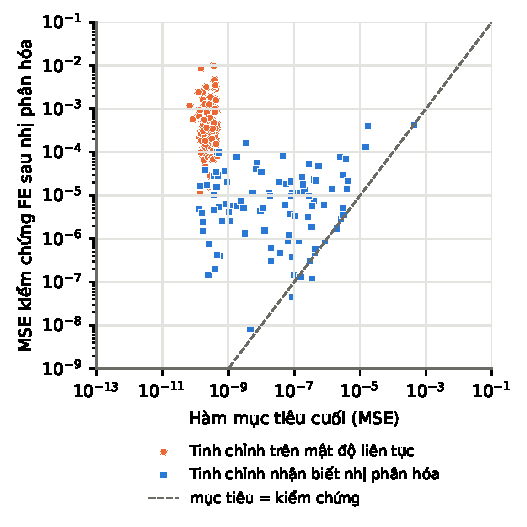
\includegraphics[width=\linewidth,height=0.72\textheight,keepaspectratio]{fig_gap_vi.pdf}
    \column{0.48\textwidth}
    \begin{itemize}
      \item Tinh chỉnh mã ẩn theo độ nhạy FE \textbf{chính xác} trên
        trường liên tục
      \item Hàm mục tiêu $\to\sim\!10^{-10}$
      \item Sai số kiểm chứng vẫn $10^{-4}$--$10^{-2}$: lớn hơn
        \textbf{sáu bậc}
      \item Bộ tối ưu khai thác mật độ xám \textbf{không sống sót qua nhị
        phân hóa}, như khai thác một surrogate sai
      \item Không nhìn thấy được trên đường cong loss
    \end{itemize}
  \end{columns}
\end{frame}

\begin{frame}{Ví dụ: cùng mã ẩn, ba cách tinh chỉnh}
  \begin{columns}[c]
    \column{0.55\textwidth}
    \centering
    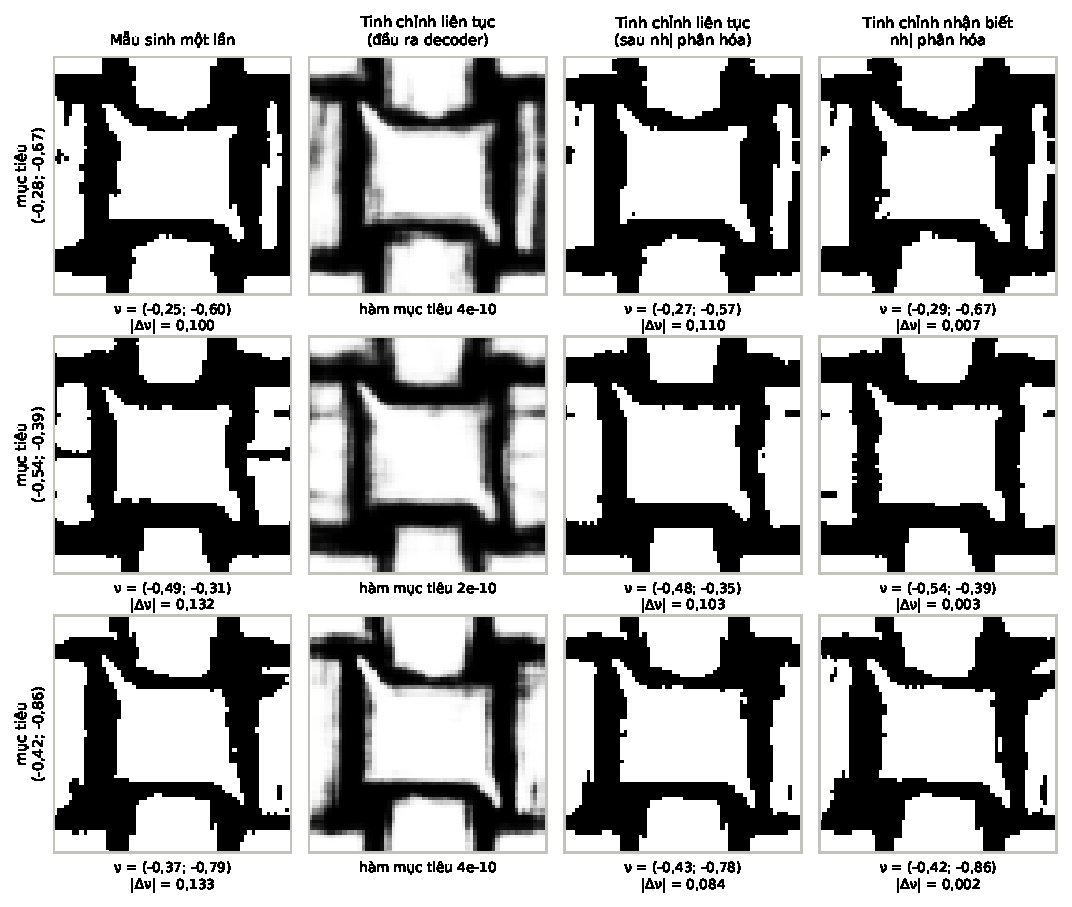
\includegraphics[width=\linewidth,height=0.82\textheight,keepaspectratio]{fig_refine_examples_vi.pdf}
    \column{0.42\textwidth}
    \begin{itemize}
      \item Mỗi hàng: một điều kiện của tập A
      \item Tinh chỉnh liên tục đạt mục tiêu trên \textbf{trường xám}
      \item Bản nhị phân hóa của nó có \textbf{tính chất khác}
      \item Tinh chỉnh nhận biết nhị phân hóa tối ưu trực tiếp thiết kế
        nhị phân
    \end{itemize}
  \end{columns}
\end{frame}

\begin{frame}{Cách sửa: tối ưu chính cái được kiểm chứng}
  \begin{itemize}
    \item Đưa phiên bản \textbf{khả vi} của các phép biến đổi kiểm chứng
      vào hàm mục tiêu:
      \begin{itemize}
        \item Phép chiếu Heaviside $H_\beta$, $\eta=0{,}5$, tăng dần
          $\beta\in\{1,4,16,64\}$ (L-BFGS khởi động lại mỗi mức)
        \item Lấy mẫu lại \texttt{nearest-exact}, khớp đúng khâu kiểm chứng
      \end{itemize}
    \item Loss $\mathcal L=\tfrac12\lVert\boldsymbol\nu-\boldsymbol\nu^{*}\rVert^2$,
      gradient $\partial\mathcal L/\partial z$ chính xác qua đồng nhất hóa
    \item Khâu kiểm chứng thay $H_\beta$ bằng ngưỡng cứng 0,5
    \item Chọn theo sai số kiểm chứng; loại ô suy biến
      ($\min E_i<10^{-3}E_0$)
  \end{itemize}
  \vspace{3mm}
  \begin{alertblock}{Không mới trong tối ưu tô-pô}
    Heaviside projection đã quen thuộc (Guest et al., 2004). Điểm mới:
    bỏ qua nó \textbf{làm đổi kết luận} khi so sánh phương pháp, và cả mô hình
    sinh lẫn SIMP đều cần nó.
  \end{alertblock}
\end{frame}

% ===========================================================================
\section{Kết quả}

\begin{frame}{Độ chính xác kiểm chứng FE (tập A, 100 mục tiêu)}
  \centering
  \small
  \begin{tabular}{llcccr}
    \toprule
    Chế độ & Tinh chỉnh & $\RR(\nuot)$ & MAE($\nuot$) & $\Delta$MAE [CI 95\%] & FE\\
    \midrule
    Mẫu đơn & không               & 0,874 & 0,0517 & -- & 1\\
            & liên tục            & 0,976 & 0,0219 & $+57,7\%$ [49; 65] & 51\\
            & nhận biết nhị phân  & \textbf{0,999} & \textbf{0,0038} & $\mathbf{+92,7\%}$ [90; 95] & 78\\
    \midrule
    Best-of-30 & không             & 0,988 & 0,0142 & -- & 30\\
               & liên tục          & 0,962 & 0,0247 & \textcolor{red!70!black}{$-73,8\%$} [$-119$; $-39$] & 79\\
               & nhận biết nhị phân & \textbf{0,998} & \textbf{0,0045} & $\mathbf{+68,3\%}$ [59; 76] & 107\\
    \bottomrule
  \end{tabular}
  \vspace{5mm}
  \begin{itemize}
    \item Tinh chỉnh liên tục còn \textbf{làm hỏng} best-of-30
    \item Tái lập trên 2 tập rời nhau: mẫu đơn $0{,}831\to0{,}989$;
      best-of-30 giảm sai số \textbf{59--68\%} trên cả 3 tập
  \end{itemize}
\end{frame}

\begin{frame}{Đồ thị tương quan: mục tiêu vs kiểm chứng}
  \centering
  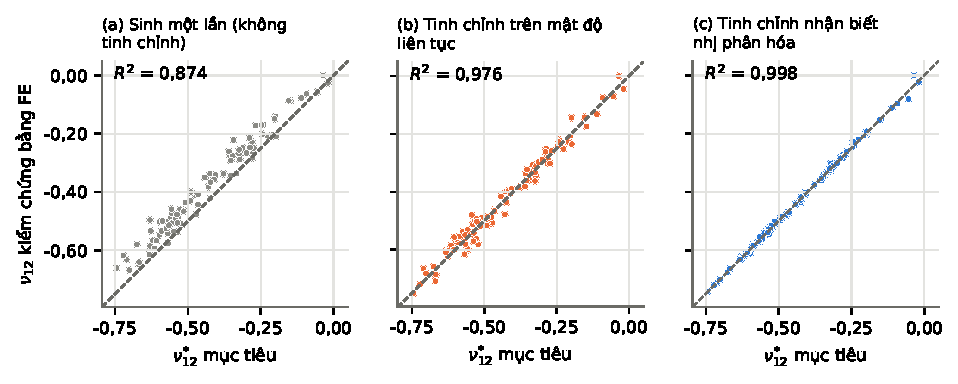
\includegraphics[width=\linewidth,height=0.68\textheight,keepaspectratio]{fig_parity_vi.pdf}\\[2mm]
  {\small (a) chưa tinh chỉnh \quad (b) tinh chỉnh liên tục \quad
  (c) tinh chỉnh nhận biết nhị phân hóa --- cùng mã ẩn khởi đầu}
\end{frame}

\begin{frame}{So với tối ưu tô-pô chạy từ đầu (cùng chuỗi kiểm chứng)}
  \centering
  \small
  \begin{tabular}{llccccc}
    \toprule
    Tập & Phương pháp & $\RR(\nuot)$ & Cặp & FE/mục tiêu & Suy biến & Chế tạo\\
    \midrule
    A & sinh & 0,998 & 0,0139 & \textbf{107} & 1 & 0,32\\
      & SIMP & 0,997 & 0,0128 & 897 & 0 & \textbf{0,77}\\
    B & sinh & 0,995 & 0,0229 & \textbf{107} & 2 & 0,35\\
      & SIMP & 0,996 & 0,0139 & 889 & 0 & \textbf{0,74}\\
    C & sinh & 0,998 & 0,0082 & \textbf{107} & 0 & 0,32\\
      & SIMP & 0,998 & 0,0126 & 893 & 0 & \textbf{0,83}\\
    \bottomrule
  \end{tabular}
  \vspace{4mm}
  \begin{itemize}
    \item SIMP: MMA + Heaviside $\beta\to64$, tốt nhất trong 4 khởi tạo
    \item Độ chính xác $\nuot$ \textbf{ngang nhau} với \textbf{$\sim$8$\times$
      ít lần giải FE}
    \item Mọi ô suy biến của cVAE đều thuộc mục tiêu dị hướng mạnh $r\ge10$
  \end{itemize}
\end{frame}

\begin{frame}{Kiểm định đặt trước trên tập mới C}
  \textbf{Tiêu chí ghi trước khi chạy} (mục tiêu $r<10$, CI 95\% ghép cặp
  không chứa 0):
  \vspace{2mm}
  \begin{center}
  \begin{tabular}{lcc}
    \toprule
    Tiêu chí & Kết quả & \\
    \midrule
    Sai số cặp $(\nuot,\nuto)$ thấp hơn SIMP & $27\%$ [8; 42] & \pass\\
    Sai số $\nuot$ thấp hơn SIMP & $19\%$ [$-10$; 40] & \fail\\
    \bottomrule
  \end{tabular}
  \end{center}
  \vspace{2mm}
  \begin{itemize}
    \item Pipeline cuối (không cân bằng cạnh): cả hai đạt trên 3 tập
      (35--41\%) --- chỉ báo như \textbf{phân tích độ nhạy}
    \item Chênh lệch $\nuot$ $\sim\!10^{-3}$ $\ll$ sai số lưới 0,015
  \end{itemize}
  \begin{block}{Claim được phép}
    Ngang SIMP hội tụ về $\nuot$ với $\sim$8$\times$ ít FE; sai số cặp thấp
    hơn với dị hướng vừa phải. \textbf{Không} claim $\nuot$ tốt hơn SIMP.
  \end{block}
\end{frame}

\begin{frame}{Thiết kế cuối: pipeline sinh vs SIMP (tập A)}
  \centering
  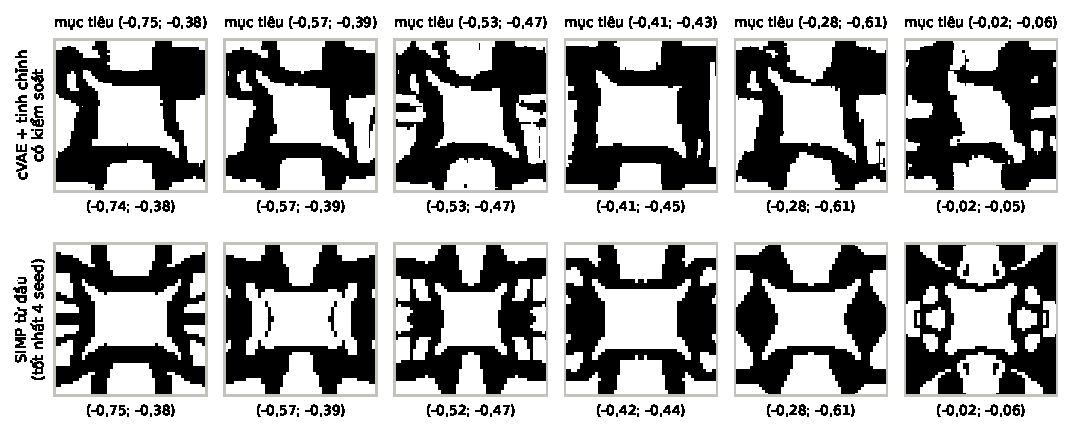
\includegraphics[width=\linewidth,height=0.8\textheight,keepaspectratio]{fig_designs_vi.pdf}\\[1mm]
  {\small Cùng mục tiêu, kèm $(\nuot,\nuto)$ mục tiêu và kiểm chứng}
\end{frame}

\begin{frame}{Chỗ pipeline sinh thua}
    \begin{itemize}
      \item \textbf{Dị hướng mạnh $r\ge10$:} kém hơn nhiều ở 4/5 mục tiêu;
        30/30 ứng viên đều đứt rời (chỉ 2,8\% dữ liệu có $r>10$)
      \item \textbf{Chế tạo:} 0,32--0,35 so với 0,74--0,83
      \item \textbf{Đổi dấu $\nu$ (OOD):} thắng truy xuất thư viện, thua
        SIMP rõ rệt
      \item \textbf{Biên độ:} bão hòa nơi dữ liệu kết thúc
      \item Lai cVAE$\to$SIMP (đặt trước): \fail{} 2/4 tiêu chí
    \end{itemize}
\end{frame}

\begin{frame}{SIMP cũng có cùng khoảng lệch}
  \begin{itemize}
    \item Cuối continuation: sai số trên trường đã chiếu trung vị
      $2\times10^{-7}$; sau ngưỡng \textbf{$3{,}6\times10^{-2}$}
    \item 57\% mục tiêu: khởi tạo tốt nhất theo trường chiếu
      \textbf{không phải} tốt nhất theo kiểm chứng
    \item Thí nghiệm đổi dấu: SIMP trả về \textbf{ô rỗng} ($\nu=\nu_0=0{,}3$)
      cho 3/28 mục tiêu --- bộ kiểm chứng không bảo vệ vẫn chấp nhận
  \end{itemize}
  \vspace{4mm}
  \begin{block}{Hệ quả}
    Chọn theo sai số kiểm chứng và kiểm tra suy biến là \textbf{bắt buộc
    cho mọi phương pháp}, không riêng mô hình sinh.
  \end{block}
\end{frame}

% ===========================================================================
\section{Khi nào dùng phương pháp nào}

\begin{frame}{Quy tắc chọn phương pháp cho người thiết kế}
  \centering
  \begin{tabular}{p{0.36\linewidth}p{0.1\linewidth}p{0.44\linewidth}}
    \toprule
    Tình huống & Dùng & Bằng chứng\\
    \midrule
    Hàng nghìn mục tiêu trong dải dữ liệu, $r<10$
      & \textbf{Sinh} & Ngang $\nuot$, $\sim$8$\times$ ít FE; sai số cặp thấp hơn 27\%\\
    Ít mục tiêu hoặc một ô & SIMP & Chi phí dữ liệu hòa vốn sau
      $\sim$3\,500 mục tiêu\\
    Dị hướng mạnh $r\ge10$ & SIMP & Sinh kém hơn nhiều ở 4/5 mục tiêu\\
    Chế tạo là bắt buộc & SIMP & 0,74--0,83 so với 0,32--0,35\\
    Đổi dấu $\nu$ / vượt biên độ & SIMP & Sinh chỉ thắng truy xuất\\
    Mọi phương pháp & -- & Tối ưu \& chọn trên thiết kế nhị phân; loại ô
      suy biến\\
    \bottomrule
  \end{tabular}
\end{frame}

\begin{frame}{Giới hạn}
  \begin{itemize}
    \item Chính xác so với mô hình FE $50\times50$; sai số lưới (0,015) lớn
      hơn sai số trung bình báo cáo --- thứ hạng giữ nguyên trên $200^2$
    \item Chỉ 2D, đàn hồi tuyến tính, $\nu_0=0{,}3$; chưa thử nghiệm thực tế
    \item Dữ liệu huấn luyện $\approx$2,7--3,0 triệu lần giải FE
    \item Phương pháp tinh chỉnh chọn sau thất bại trên tập A; tái lập B, C
      và kiểm định đặt trước giảm nhưng không xóa phụ thuộc này
  \end{itemize}
\end{frame}

\begin{frame}{Kết luận}
  \begin{enumerate}
    \item cVAE + tinh chỉnh nhận biết nhị phân hóa là \textbf{bộ giải thiết kế
      ngược auxetic} ngang SIMP hội tụ với $\sim$8$\times$ ít FE, tái lập trên
      3 tập
    \item Chìa khóa: tính hàm mục tiêu trên \textbf{chính thiết kế sẽ được
      kiểm chứng} --- nhị phân, lấy mẫu lại, kiểm suy biến
    \item Phạm vi rõ ràng: dùng mô hình sinh cho nhiều mục tiêu, dị hướng
      vừa phải; còn lại dùng SIMP
    \item Nguyên tắc áp dụng cho cả SIMP
  \end{enumerate}
  \vspace{4mm}
  \textbf{Đích nộp:} Structural and Multidisciplinary Optimization
\end{frame}

\begin{frame}
  \centering
  \vfill
  {\Huge Cảm ơn thầy và mọi người!}\\[6mm]
  {\large Hỏi \& đáp}
  \vfill
\end{frame}

\end{document}
